\clearpage
\section*{\currfilename}

\begin{figure}[H]
  \fontsize{10pt}{10pt}\selectfont
  \begin{center}
    %\resizebox{3.0in}{1.0in}{
    \begin{tikzpicture}[auto, scale=1.0, every node/.style={transform shape}, node distance=0.6cm,>=latex']
      \matrix[ampersand replacement=\&, row sep=0cm, node distance=4.0cm] (regions) at (0,0) {
      \node [draw=black, label=below:{\shortstack[c]{GHV Equations\\ of Motion}}, label=above:{$A,B\Lambda,C$},  minimum width=3cm, inner sep=0mm] (block3){\centering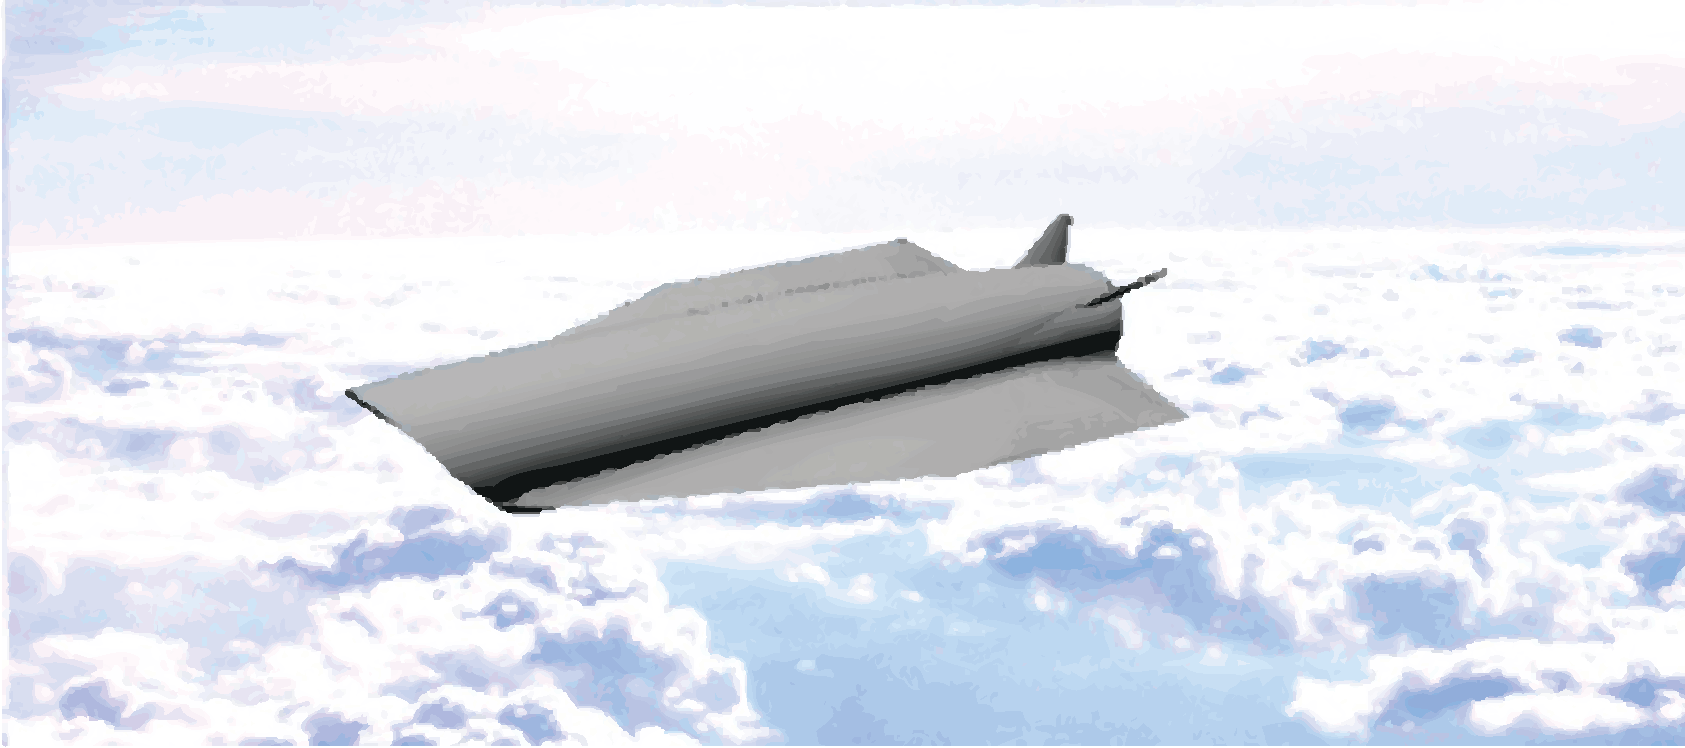
\includegraphics[width=4cm]{../fig/ghvclouds.pdf}}; \\
      };
      %\matrix[ampersand replacement=\&, row sep=0.6cm, left of=block3, node distance=5.0cm] (xxxx) {
      %\node [squareblock, minimum width=2cm] (block1) {Baseline};\\
      %%\node [block, minimum width=2cm] (block2) {\shortstack{Adaptive \\ Augmentation}};\\
      %};
      \node[block,left of=block1, node distance=4.0cm](node1) {};
      %\node [squareblock, minimum width=2cm] (block2) {\shortstack{Adaptive \\ Augmentation}};
      %\draw [<-] (block3.west) + (0cm,0.6cm) -- (block1);
      %\draw [<-] (block3.west) + (0cm,-0.6cm) -- (block2);
      %
      %\draw [->] (R1.east) + (0cm,-0.5cm) -- node [block,pos=0.95]{$y$} (output2);
      %\node[input, below of=block2,node distance=1.5cm](input4){};
      %draw
      %\draw [<-] (block2.west) + (0cm,0.3cm) -- node [block]{test} (block1);

      %\draw [<-] (block2.west) + (0cm,0.3cm) -- node [near end]{$z_{\text{cmd}}$} (b2out1);
      %\draw [<-] (block2.west) + (0cm,-0.3cm) -- node [near end]{$y$} (b2out2);
      %\draw [->] (R1outx) -- node [pos=0.9]{} (output1);
      %\draw [->] (block2) -- node [near start]{$u$} (R1);
      %\draw [->] (input2) -- node [near start]{bias} (R1outx);
      %\draw [->] (R1.east) + (0cm,0.5cm) -- (R1outx);
      %\draw [->] (R1outx) -- node [pos=0.9]{} (output1);
      %\draw [->] (R1.east) + (0cm,-0.5cm) -- node [pos=0.95]{$y$} (output2);
      %\draw [->] (input4) -- node [near start]{$S_{1}$, $L$} (block2);
      %cross out
      %\coordinate (arrow1) at ([xshift=-0.4cm,yshift=-0.3cm] output1);
      %\coordinate (arrow2) at ([xshift=0.2cm,yshift=0.3cm] output1);
      %\coordinate (arrow3) at ([xshift=-0.4cm,yshift=0.3cm] output1);
      %\coordinate (arrow4) at ([xshift=0.2cm,yshift=-0.3cm] output1);
      %\draw[-,red,line width=2](arrow1) -- (arrow2);
      %\draw[-,red,line width=2](arrow3) -- (arrow4);
    \end{tikzpicture}
    %}
  \end{center}
\end{figure}
